\chapter{Schulze Method : Evidence Carrying Computation}
\label{cha:schulze_method}
%Same as the last chapter, introduce the motivation and the high-level picture to
%readers, and introduce the sections in this chapter.

\epigraph{The negligence of a few could easily send a ship to the bottom, but if it has the wholehearted 
co-operation of all on board it can be safely brought to part.} 
{\textit{Sardar Vallabhbhai Patel}} 

\section{Introduction}
 Correctness and verifiability/evidence are two main pillar of any democratic election. 
 In case of paper ballot election, correctness and verifiability of counting is achieved 
 by public scrutiny because each step is carefully observed by general member of public, 
 agents from different political parties. For example. casting ballot at booth 
 is carefully observed by polling agents and 
 counting ballots is observed by the scrutineers appointed by different political parties \ref{fig:scrutineers}.
 Given that electronic voting is relatively young, in this chapter we investigate 
 how to achieve the correctness and verifiability similar to paper ballot election.
 
\begin{figure}[h!]
 \centering
  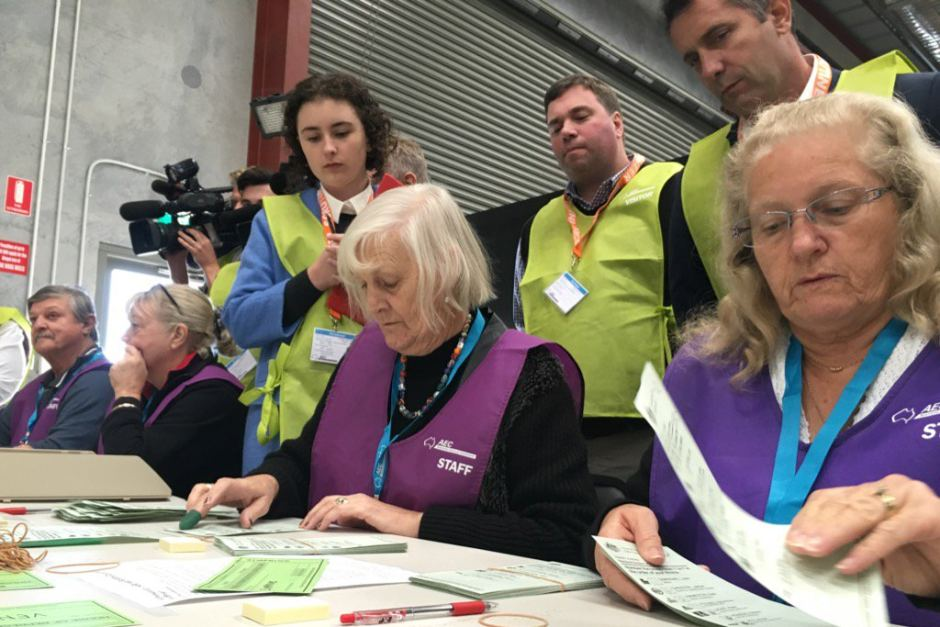
\includegraphics[width=1\linewidth]{figs/scrutineers.jpg}
  \caption{Scrutineers, in green jacket, observing the ballot counting}
  \label{fig:scrutineers}
  \end{figure} 
 
 
 
 \textbf{Chapter overview:} In this chapter, we explain the Schulze method in section \ref{sec:schulze_algorithm}, 
 and its formal specification in the section \ref{sec:spec}. The  corner stone of our formalization is 
 a correct by construction dependent inductive data type 
 that represents all correct executions (\ref{sec:inductive_type}) with the formal proof of
 that every Schulze election have winners (\ref{sec:all_winners}).  Every inhabitant of 
 this dependent inductive data type not only produces a final result, but also all the 
 intermediate steps which lead to the notion of evidence or scrutiny sheet (section 
  \ref{sec:scrunity_sheet}).  In the section \ref{sec:count_million}, we discuss the optimization techniques
   to overcome the deficiencies in extracted Haskell code from Coq formalization. Based on 
   these optimizations, the extracted Haskell code was able to count millions of ballots in few 
   minutes. 
   Finally, we conclude the chapter in the section \ref{sec:discussion} with 
   the achievements and drawbacks of our work on the scale of \textit{Correctness},
   \textit{Privacy}, and \textit{Verifiability}.
 



\section{Schulze Algorithm}
\label{sec:schulze_algorithm}
The Schulze Method \citep{Schulze:2011:NMC} is a vote counting scheme
that elects a single winner, based on preferential votes. 
The method itself rests on the relative 
\emph{margins} between two candidates, i.e. the number of
voters that prefer one candidate over another.  The margin induces
an ordering between candidates, where a candidate $c$ is more
preferred than $d$, if more voters prefer $c$ over $d$ than 
vice versa. One can construct simple examples (see e.g.
\citep{Rivest:2010:OSW}) where this order does not have a maximal
element (a so-called \emph{Condorcet Winner}). Schulze's observation
is that this ordering \emph{can} be made transitive by considering
sequences of candidates (called \emph{paths}). Given candidates $c$
and $d$, a \emph{path} between $c$ and $d$ is a sequence of candidates
 $p = (c, c_1,\dots, c_n, d)$ that joins $c$ and $d$, and 
 the \emph{strength} of a
path is the minimal margin between adjacent nodes. This induces the
\emph{generalised margin} between candidates $c$ and $d$ as the
strength of the strongest path that joins $c$ and $d$. A candidate
$c$ then wins a Schulze count if the generalised margin between $c$
and any other candidate $d$ is at least as large as the generalised
margin between $d$ and $c$. More concretely:

\begin{itemize}

\item Consider an election with a set of $m$ candidates
 $C$ = $\{c1,\dots,cm\}$, and 
	a set of $n$ votes $P$ = $\{b1,\dots,bn\}$. A vote
	is represented as function $b: C \rightarrow \mathbb{N}$ that 
	assigns natural 
	number (the preference) to each candidate. We recover a strict linear  
	preorder $<_b$ on candidates by setting $c <_b d$ if $b(c) > b(d)$. 
	
\item Given a set of ballots $P$ and candidate set $C$, we construct graph $G$ based on the margin function $m: C \times C \to \mathbb{Z}$. Given two candidates $c, d \in C$,
the \emph{margin} of $c$ over $d$ is
the number of voters that prefer $c$ over $d$, minus the number of voters that prefer $d$ over $c$. 
In symbols:
\[
  m(c, d) = \sharp \lbrace b \in P \mid c >_b d \rbrace -
            \sharp \lbrace b \in P \mid d >_b c \rbrace
\] where $\sharp$ denotes cardinality and $>_b$ is the strict
(preference) ordering given by the ballot $b \in P$.





\item A directed \emph{path} in the graph, $G$, from
candidate $c$ to candidate $d$ is a sequence $p \equiv c_0, \dots, c_{n+1}$
of candidates with $c_0 = c$ and $c_{n+1} = d$ ($n \geq 0$), and the
\emph{strength}, st, of path, p, is the minimum margin of adjacent
nodes, i.e.
\[ st(c_0, \dots, c_{n+1}) = \min \lbrace m (c_i, c_{i+1}) \mid 0
\leq i \leq n \rbrace. \]
\item For candidates c and d, let $M(c, d)$ denote the maximum strength, or generalized margin of a path
	from c to d i.e. 
	\[ M(c, d) = \max \lbrace st (p) : \text{p is path from c to d in G} \rbrace\]
	
\item The winning set is, always non empty and  formally proved in \ref{sec:all_winners}, defined as 
 \[ W =  \lbrace c \in C : \forall d \in C \setminus \{c\}, M (c, d) \geq M (d, c) \rbrace\]

\end{itemize}

The Schulze method
stipulates that a candidate $c \in C$ is a \emph{winner} of the
election with margin function $m$ if, for all other candidates $d \in
C$, there exists a number $k \in Z$ such that
\begin{itemize}
\item there is a path $p$ from $c$ to $d$ with strength $st(p) \geq k$
\item all paths $q$ from $d$ to $c$ have strength $st(q) \leq k$.
\end{itemize}
Informally speaking, we can say that  candidate $c$
\emph{beats} candidate $d$ if there's a path $p$ from
$c$ to $d$ which stronger than any path from $d$ to $c$. Using
this terminology, a candidate $c$ is a winner if $c$ cannot be
beaten by any (other) candidate.


	\subsection{An Example}
	For some given set of ballots (the actual set of ballots are not very important because we want to demonstrate the Condercet Paradox), we have computed 
	the margin function $m$ such that $m$ ($A, B$) = 3, $m$ ($B, A$) = -3, $m$ ($A, C$) = -1, 
	$m$ ($C, A$) = 1, $m$ ($B, C$) = 5, and $m$ ($C, B$) = -5. We have drawn the graph below, and 
	it shows that collective can be cyclic, even if the preferences of individual voters are not cyclic. This phenomena 
	is known as Condercet paradox and first observed by french philosopher Marquis de Condorcet in late 18th century \footnote{https://gallica.bnf.fr/ark:/12148/bpt6k417181}.
	     
\[
\xymatrix@R=12ex@C=12ex{
A \ar@/^/[rr]^{3} \ar@/_/[dr]_{-1} & & B \ar@/^/[ll]^{-3}
\ar@/^/[dl]^5 \\
& C \ar@/_/[ul]_{1} \ar@/^/[ur]^{-5}
}\]

The main idea of the method is to resolve cycles by considering \emph{transitive preferences} or a generalised notion of margin. Below is the graph $M$, generalize 
margin (sometimes, we use generalize margin matrix or generalize margin function) after running  the Schulze method on margin function $m$.  In order to 
compute $M(A, B)$, we first compute all the path from candidate $A$ to $B$. Well, we have just two path from $A$ to $B$, a direct path between them and 
a intermediate path via candidate $C$.  Now that we two paths, we compute the path strength $st$ for each path, $st(A, B) = min \lbrace m (A, B) \rbrace $ 
and $st (A, C, B)$ = $min \lbrace m (A, C), m (C, B) \rbrace$.  Simply these expression:

\begin{align}
st (A, B)&=  \min \lbrace m (A, B) \rbrace  \nonumber \\
					  &= \min \lbrace 3 \rbrace \nonumber \\
                     &= 3 \nonumber
\end{align}


\begin{align}
st (A, C, B)&=  \min \lbrace m (A, C), m (C, B) \rbrace  \nonumber \\
                     &= \min \lbrace -1, -5 \rbrace \nonumber \\
                     &= -5\nonumber
\end{align}

Once we have the path strength for every path between $A$ and $B$, we compute generalize margin 
$M(A, B) = \max \lbrace st (A, B), st(A, C, B) \rbrace$, and simplification leads to 3; hence the arrow going
$A$ to $B$ has strength 3.  


\begin{align}
M (A, B)&=  \max \lbrace st (A, B), st(A, C, B) \rbrace \nonumber \\
                     &= \max \lbrace 3, -5 \rbrace \nonumber \\
                     &= 3\nonumber
\end{align}

Similarly, we can compute other values as well. 

\begin{align}
\hspace*{-10mm} st (B, A)&=  \min \lbrace m (B, A) \rbrace  \nonumber \\
					  &= \min \lbrace -3 \rbrace  \nonumber \\
                     &= -3 \nonumber
\end{align}


\begin{align}
st (B, C, A)&=  \min \lbrace m (B, C), m (C, A) \rbrace  \nonumber \\
                     &= \min \lbrace 5, 1 \rbrace \nonumber \\
                     &= 1\nonumber
\end{align}

\begin{align}
M (B, A)&=  \max \lbrace st (B, A), st(B, C, A) \rbrace \nonumber \\
                     &= \max \lbrace -3, 1 \rbrace \nonumber \\
                     &= 1\nonumber
\end{align}

\begin{align}
st (A, C)&=  \min \lbrace m (A, C) \rbrace  \nonumber \\
					  &= \min \lbrace -1 \rbrace  \nonumber \\
                     &= -1 \nonumber
\end{align}


\begin{align}
st (A, B, C)&= \min \lbrace m (A, B), m (B, C) \rbrace  \nonumber \\
                     &= \min \lbrace 3, 5 \rbrace \nonumber \\
                     &= 3\nonumber
\end{align}

\begin{align}
M (A, C)&=  \max \lbrace st (A, C), st(A, B, C) \rbrace \nonumber \\
                     &= \max \lbrace -1, 3 \rbrace \nonumber \\
                     &= 3\nonumber
\end{align}


\begin{align}
st (C, A)&=  \min \lbrace m (C, A) \rbrace  \nonumber \\
					  &= \min \lbrace 1 \rbrace  \nonumber \\
                     &= 1 \nonumber
\end{align}


\begin{align}
st (C, B, A)&= \min \lbrace m (C, B), m (B, A) \rbrace  \nonumber \\
                     &= \min \lbrace -5, -3 \rbrace \nonumber \\
                     &= -5\nonumber
\end{align}

\begin{align}
M (C, A)&=  \max \lbrace st (C, A), st(C, B, A) \rbrace \nonumber \\
                     &= \max \lbrace 1, -5 \rbrace \nonumber \\
                     &= 1\nonumber
\end{align}





\begin{align}
st (C, B)&=  \min \lbrace m (C, B) \rbrace  \nonumber \\
					  &= \min \lbrace -5 \rbrace  \nonumber \\
                     &= -5 \nonumber
\end{align}


\begin{align}
st (C, A, B)&= \min \lbrace m (C, A), m (A, B) \rbrace  \nonumber \\
                     &= \min \lbrace 1, 3\rbrace \nonumber \\
                     &= 1\nonumber
\end{align}

\begin{align}
M (C, B)&=  \max \lbrace st (C, B), st(C, A, B) \rbrace \nonumber \\
                     &= \max \lbrace -5, 1 \rbrace \nonumber \\
                     &= 1\nonumber
\end{align}


\begin{align}
st (B, C)&=  \min \lbrace m (B, C) \rbrace  \nonumber \\
					  &= \min \lbrace 5 \rbrace  \nonumber \\
                     &= 5 \nonumber
\end{align}


\begin{align}
st (B, A, C)&= \min \lbrace m (B, A), m (A, C) \rbrace  \nonumber \\
                     &= \min \lbrace -3, -1\rbrace \nonumber \\
                     &= -3\nonumber
\end{align}

\begin{align}
M (B, C)&=  \max \lbrace st (B, C), st(B, A, C) \rbrace \nonumber \\
                     &= \max \lbrace 5, -3 \rbrace \nonumber \\
                     &= 5\nonumber
\end{align}

\noindent
Now we have computed all the values of generalize margin $M$, we can interpret it as 
graph show below.  It is clear for the graph that candidate $A$ is winner, as he beats 
$B$ with strength 3 (reverse path from $B$ to $A$ is weaker, i.e. strength 1) and 
$C$ with strength 3 (reverse path from $C$ to $A$ is weaker, i.e. strength 1). 

\[
 \xymatrix@R=12ex@C=12ex{
A \ar@/^/[rr]^{3} \ar@/_/[dr]_{3} & & B \ar@/^/[ll]^{1}
\ar@/^/[dl]^5 \\
& C \ar@/_/[ul]_{1} \ar@/^/[ur]^{1}
}\]
	 
	
	
\section{Formal Specification} \label{sec:spec}
	We start our Coq formalization assuming finite  and non-empty 
	set of candidates. Also, we assume decidable equality on 
	candidates. For our purposes, the
	easiest way of stipulating that a type be finite is to require
	existence of a list containing all inhabitants of this type \citep{DBLP:conf/icfp/FirsovU15}.

\begin{verbatim}
  Variable cand : Type.
  Variable cand_all : list cand.
  Hypothesis cand_fin : forall c: cand, In c cand_all.
  Hypothesis dec_cand : forall n m : cand, {n = m} + {n <> m}.
  Hypothesis cand_in : cand_all <> nil.
\end{verbatim}

\noindent
For the specification of winners of Schulze elections, we take the
margin function as given for the moment (and later construct it from
the incoming ballots). In Coq, this is conveniently expressed as a
variable:
\begin{verbatim}
   Variable marg : cand -> cand -> Z.
\end{verbatim}

\noindent
We formalise the notion of path and strength of a path by means of a
single (but ternary) inductive proposition that asserts the
existence of a path of strength $\geq k$ between two candidates, for
$k \in Z$. The notion of winning candidate is that it beats every other candidate, i.e.  all the paths from 
the winner to other candidates are at least as strong as the reverse path. Dually, the notion of loser
 is that there is a candidate who beats the loser, i.e. the path from the candidate to the loser is 
 stronger than the reverse path. 


\begin{verbatim}
  (* prop-level path *)
  Inductive Path (k: Z) : cand -> cand -> Prop :=
    | unit c d : marg c d >= k -> Path k c d
    | cons  c d e : marg c d >= k -> Path k d e -> Path k c e.
    
  (* winning condition of Schulze Voting *)
  Definition wins_prop (c: cand) := forall d: cand, exists k: Z,
      Path k c d /\ (forall l, Path l d c -> l <= k).

  (* dually, the notion of not winning: *)
  Definition loses_prop (c : cand) := exists k: Z, exists  d: cand,
      Path k d c /\ (forall l, Path l c d -> l < k).
\end{verbatim}


\noindent
We reflect the fact that the above are \emph{propositions} in
the name of the definitions, in anticipation of type-level
definitions of these notions later. The reason for having a \textit{Prop} level definition is that 
 it is very easy  and intuitive for human to inspect the definitions, and ascertain the correctness of formalization.
As we discussed in the
\textbf{Type vs. Prop} (section \ref{sec:typeprop}), the main reason 
for having an equivalent
type-level versions of the above is that purely propositional
information is discarded during program extraction, unlike
the type-level notions of winning and losing that represent evidence
of the correctness of the determination of winners. Our goal is to 
not only compute winners and losers according to the
definition above, but also to provide independently verifiable
evidence, a scrutiny sheet or certificate, of the correctness of our computation.
The propositional
definitions of winning and losing above serve as a reference to
calibrate their type level counterparts, and we demonstrate the
equivalence between propositional and type-level conditions in the
next section. 


\label{sec:prop-type}
One of the fundamental question about the declaring some one 
as a winner or loser is that 
how can we know that, say, a candidate $c$ in fact wins a
Schulze election, and that, say, $d$ is not a winner? One possible 
answer is simply  re-run an independent implementation of the method
(usually hoping that results would be confirmed). But what happens
if results diverge?  

One major aspect of our work is that we can answer this question
by not only computing the set of winners, but in fact presenting
\emph{evidence} for the fact that a particular
candidate does or does not
win. This is a re-emphasis on \emph{Correctness},
and convincing to all, specifically to losers, leaving  no ground for speculation. 
As we stated earlier that in the context of
electronic vote counting, this is known as a
\emph{scrutiny sheet, or certification}: a tabulation of all relevant data that allows
us to verify the election outcome.
Again drawing on an already computed margin function, to
demonstrate that a candidate $c$ wins, we need to exhibit an integer
$k$ for all competitors $d$, together with
\begin{itemize}
  \item evidence for the existence of a path from $c$ to $d$ with
  strength $\geq k$
  \item evidence for the non-existence of a path from $d$ to $c$
  that is stronger than $k$
\end{itemize}


\noindent
The first item is straight forward, as a path itself is evidence for the
existence of a path, and the notion of path is inductively defined.
For the second item, we need to produce evidence of membership in
the \emph{complement} of an inductively defined set.

Mathematically, given $k \in Z$ and a margin function $m: C \times C
\to Z$, the pairs $(c, d) \in C \times C$ for which there exists a
path of strength $\geq k$ that joins both are precisely the elements
of the least fixpoint $LFP(V_k)$ of the monotone operator $V_k:
Pow(C \times C) \to Pow(C \times C)$, defined by
\[ V_k(R) = \lbrace (c, e) \in C \mid m(c, e) \geq k \mbox{ or }
(m(c, d) \geq k \mbox{ and } (d, e) \in R \mbox{ for some } d \in C)
\rbrace \]
It is easy to see that this operator is indeed monotone, and that
the least fixpoint exists, e.g. using Kleene's theorem
\citep{Stoltenberg-Hansen:1994:MTD}.  To show that there is \emph{no}
path between $d$ and $c$ of strength $> k$, we therefore need to
establish that
$(d, c) \notin LFP(V_{k+1})$.

By duality between least and greatest fixpoints, we have that \[
(c, d) \in C \times C
\setminus LFP(V_{k+1}) \iff (c,d) \in GFP(W_{k+1}) \]
where for arbitrary $k$, $W_k: Pow(C \times C) \to Pow(C \times C)$ is the operator dual
to $V_k$, i.e.
\[ W_k(R) = C \times C \setminus (V_k (C\times C \setminus R)) \]
and $GFP(W_k)$ is the greatest fixpoint of $W_k$.
As a consequence, to demonstrate that there is \emph{no} path of
strength $> k$ between candidates $d$ and $c$, we need to
demonstrate that $(d, c) \in GFP(W_{k+1})$. By the Knaster-Tarski fixpoint
theorem \citep{Tarski:1955:LTF}, this greatest fixpoint is the supremum of all
$W_{k+1}$-coclosed sets, that is, sets $R \subseteq C \times C$ for which
$R \subseteq W_{k+1}(R)$.
That is, to demonstrate that $(d, c) \in GFP(W_{k+1})$, we need
to exhibit a $W_{k+1}$-coclosed set $R$ with $(d, c) \in R$.
If we unfold the definitions, we have
\[ W_k(R) = \lbrace (c, e) \in C^2 \mid m(c, e) < k \mbox{ and
} (m(c, d) < k \mbox{ or } (d,e) \in R \mbox{ for all } d \in C)
\rbrace \]
so that given \emph{any} fixpoint $R$ of $W_k$ and $(c, e) \in W$, we
know that (i) the margin between $c$ and $e$ is $< k$ so that
there's no path of length $1$ between $c$ and $e$, and (ii) for any
choice of midpoint $d$, either the margin between $c$ and $d$ is $<
k$ (so that $c, d, \dots$ cannot be the start of a path of strength
$\geq k$) or we don't have a path between $d$ and $e$ of strength
$\geq k$. We use the following terminology:

\begin{definition} Let $R \subseteq C \times C$ be a subset and $k \in
Z$. Then $R$ is \emph{$W_k$-coclosed}, or simply
\emph{$k$-coclosed}, if $R \subseteq W_k(R)$.
\end{definition}

\noindent
Mathematically, the operator $W_k$ acts on subsets of $C \times C$
that we think of as predicates. In Coq, we formalise these
predicates as boolean valued functions and obtain the following
definitions where we isolate the function \texttt{marg\_lt} (that
determines whether the margin between two candidates is less than a
given integer) for clarity:

\begin{verbatim}
  Definition marg_lt (k : Z) (p : (cand * cand)) :=
    Zlt_bool (marg (fst p) (snd p)) k.

  Definition W (k : Z) (p: cand * cand -> bool) (x: cand * cand) :=
    andb  (marg_lt k x)
    (forallb (fun m => orb (marg_lt k (fst x, m)) 
                           (p (m, snd x))) cand_all).
\end{verbatim}

\noindent
In order to formulate type-level definitions, we need to promote the
notion of path from a Coq proposition to a proper type, and
formulate the notion of $k$-coclosed predicate.

\begin{verbatim} 
  Definition coclosed (k : Z) (f : (cand * cand) -> bool) :=
    forall x, f x = true -> W k f x = true.

  Inductive PathT (k: Z) : cand -> cand -> Type :=
  | unitT : forall c d, marg c d >= k -> PathT k c d
  | consT : forall c d e, marg c d >= k -> PathT k d e -> PathT k c e.
 
\end{verbatim}


\noindent
Now, we have following type-level definition of winning (and dually, 
no-winning) for Schulze counting. As we see that these definition not only produces 
the result, but they also produce witness, e.g. the \texttt{wins\_type} definition 
states that if a candidate, say $c$, is the winner,  
then for each individual candidates participating in election, it produces two witness:
(i) a path from itself to the beating candidate of certain strength, say $k$, and 
(ii) a $k$+1 co-closed set.  These witness are basic building blocks of the 
scrutiny sheet we produce after election. 

\begin{verbatim}
  Definition wins_type c := forall d : cand, existsT (k : Z),
    ((PathT k c d) * (existsT (f : (cand * cand) -> bool),
      f (d, c) = true /\ coclosed (k + 1) f))%type.

  Definition loses_type (c : cand) := existsT (k : Z) (d : cand),
    ((PathT k d c) * (existsT (f : (cand * cand) -> bool),
      f (c, d) = true /\ coclosed k f))%type.
\end{verbatim}

\noindent
We have two definitions of winning, \texttt{wins\_prop} which is easier for a human to inspect; 
on the other hand, \texttt{wins\_type} which is useful for the machine. 
We close the gap by formally establishing that type level winning and prop level winning 
(dually, not winning) are in fact equivalent. 

\begin{verbatim}
 Lemma wins_type_prop : forall c, wins_type c -> wins_prop c.

 Lemma wins_prop_type : forall c, wins_prop c -> wins_type c.
 
 Lemma loses_type_prop : forall c, loses_type c -> loses_prop c.
 
 Lemma loses_prop_type : forall c, loses_prop c -> loses_type c.
\end{verbatim}

\noindent
The different nature of the two propositions does not allow
us to claim an equivalence between both notions, as Coq defines
bi-implication only on propositions.

The proof of the first statement, $wins\_type\_prop$, is completely straight forward, as
the type, $win\_type$, carries all the information needed to establish the
propositional winning, $wins\_prop$. However, for the second statement 
$wins\_prop\_type$, Coq does not allow the 
case analysis or induct on a term of sort \texttt{Prop} when the sort of goal 
is not in \texttt{Prop}. We follow the techniques that we have described in 
\texttt{Type vs Prop} section (\ref{sec:reification}).
%
%This is necessary to ensure that the extraction is 
%safe process (recall that every term in sort \texttt{Prop} is erased during the extraction). 
%We followed a very similar technique described in \citep{Bertot:2004:ITP} 
%\citep{ConstructiveEpsilon}. 
\noindent
To prove the second statement, we first introduced an 
intermediate lemma based on the \emph{iterated margin
function}
$M_k: C \times C \to Z$. Intuitively, $M_k (c, d)$ is the
strength of the strongest path between $c$ and $d$ of length $\leq
k+1$. Formally,
$M_0 (c, d) = m(c, d)$ and
\[ M_{i+1}(c, d) = \max \lbrace M_i(c, d), \max \lbrace  \min
\lbrace m(c, e), M_i(e, d) \mid e \in C \rbrace \rbrace \rbrace
\] for $i \geq 0$. 
It is intuitively clear (and we establish this fact formally) that
the iterated margin function stabilises at the $n$-th iteration
(where $n$ is the number of candidates), as paths with repeated
nodes don't contribute to maximising the strength of a path. This
proof loosely follows the evident pen-and-paper proof given for
example in
\citep{Carre:1971:ANR} that is based on cutting out segments of paths
between repeated nodes and so reaches a fixed point.

\begin{verbatim}
 Lemma iterated_marg_fp: forall (c d : cand) (n : nat),
      M n c d <= M (length cand_all) c d.
\end{verbatim}


\noindent
That is, the \emph{generalised margin}, i.e. the strength of the strongest (possibly infinite) path
between two candidates is effectively computable.

This allows us to relate the propositional winning conditions to the
iterated margin function and showing that a candidate $c$ is winning
implies that the generalised margin between this candidate and any
other candidate $d$ is at least as large as the generalised margin between $d$
and $c$.

\begin{verbatim}
  Lemma wins_prop_iterated_marg (c : cand) : wins_prop c ->
      forall d, M (length cand_all) d c <= M (length cand_all) c d.
\end{verbatim}

\noindent
This condition on iterated margins can in turn be used to establish the
type-level winning condition, thus closing the loop to the type
level winning condition.

\begin{verbatim}
  Lemma iterated_marg_wins_type (c : cand) : (forall d,
      M (length cand_all) d c <= M (length cand_all) c d) ->
      wins_type c.
\end{verbatim}

Similarly, we connect the propositional losing to type level losing via generalized margin. We show that 
candidate $c$ is losing then there is a candidate $d$ and generalized margin between candidate $d$ and 
$c$ is more that generalized margin between $c$ and $d$.  Using this fact, we can prove the 
type level losing condition. 

\begin{verbatim} 
  Lemma loses_prop_iterated_marg (c : cand):
      loses_prop c ->
      (exists d, M (length cand_all) c d < M (length cand_all) d c).

  Lemma iterated_marg_loses_type (c : cand) :
      (exists d, M (length cand_all) c d < M (length cand_all) d c) 
      -> loses_type c.
\end{verbatim}


The proof of lemma  $iterated\_marg\_loses\_type$ is not straight forward because
we are in a similar situation  as we were in $wins\_prop\_type$. 
We can not eliminate \texttt{exists n, P n} in order to show \texttt{existsT n, P n},
because Coq would not allows to do case analysis on \texttt{exists n, P n} (a term of 
type \texttt{Prop}) since the goal, \texttt{existsT n, P n} (a term of type \texttt{Type}), is not in
\texttt{Prop}. We again follow the technique described in 
\texttt{Type vs Prop} section (\ref{sec:reification}).
We do  a linear search on list of candidates  to find the witness constructively, and since, 
the list of candidates is  finite we would eventually terminate and find one.  
This completes our loop of prop level loser to type level loser. 


\begin{verbatim}
Corollary reify_opponent (c: cand):
  exists  d, M  (length cand_all) c d < M (length cand_all) d c ->
  existsT d, M  (length cand_all) c d < M (length cand_all) d c.
\end{verbatim}



\noindent
The crucial part of establishing the type-level winning conditions
in the proof of the lemma above is the construction of a co-closed set. 
First note that \texttt{M (length cand\_all)} is precisely
the generalised margin function. Writing $g$ for this function, we
assume that $g(c, d) \geq g(d, c)$ for all candidates $d$, and given
$d$, we need to construct a $k+1$-coclosed set $S$ where $k = g(c, d)$.
One option is to put
$S = \lbrace (x, y) \mid g(x, y) < k+1 \rbrace$. As every
$i$-coclosed set is also $j$-coclosed for $i \leq j$, the set $S' =
\lbrace (x, y) \mid g(x, y) < g(d, c) + 1 \rbrace$ is also
$k+1$-coclosed and (in general) of smaller cardinality. We therefore
witness the existence of a $k+1$-coclosed set with $S'$ as this
leads to certificates that are smaller in size and therefore easier
to check.

We note that the difference between the type-level and the
propositional definition of winning 
is in fact more than a mere reformulation. As remarked before, one
difference is that purely propositional evidence is erased during
program extraction so that using just the propositional definitions,
we would obtain a determination of election winners, but no
additional information that substantiates this (and that can be
verified independently). The second difference is conceptual: it is
easy to verify that a set is indeed coclosed as this just involves a
finite (and small) amount of data, whereas the fact that \emph{all} paths
between two candidates don't exceed a certain strength is impossible
to ascertain, given that there are infinitely many paths.

In summary, determining that a particular candidate wins an election
based on the \texttt{wins\_type} notion of winning, the extracted
program will \emph{additionally} deliver, for all other candidates,
\begin{itemize}
\item an integer $k$ and a path of strength $\geq k$ from the winning candidate to the
other candidate 
\item a co-closed set that witnesses that no path of strength $>k$
exists in the opposite direction.
\end{itemize}

\noindent
It is precisely this additional data, which we call scrutiny sheet,
(on top of merely declaring a set of
election winners) that allows for scrutiny of the process, as it
provides an orthogonal approach to verifying the correctness of the
computation: both checking that the given path has a certain
strength, and that a set is indeed co-closed, is easy to verify.
We reflect more on this in Section
\ref{sec:discussion}, and present an example of a full scrutiny
sheet in the next section, when we join the type-level winning
condition with the construction of the margin function from the
given ballots. 
\iffalse
\ref{sec:discussion}. In a nutshell, the correctness of the
computation of the (set of) winner(s) can be cross-checked by
checking whether
\begin{itemize}

\end{itemize}
\item the path provided is really a path of the claimed strength
\item the set provided is indeed co-closed
\end{itemize}

\noindent
For this verification to indeed reflect that the set of winners is
as claimed, we formally establish that both notions are provably
equivalent. It is relatively simple to establish the propositional
winning conditions from the type-level ones. The converse is
slightly harder.
\fi


\subsection{Vote Counting as Inductive Type}
\label{sec:inductive_type}
Up to now, we have described the specification of Schulze voting
relative to a given margin function. We now describe the
specification (and computation) of the margin function given a
profile (set) of ballots.  Our formalisation describes an individual
\emph{count} as a type with the interpretation that all inhabitants
of this type are correct executions of the vote counting algorithm.
In the original paper describing the
Schulze method \citep{Schulze:2011:NMC}, a ballot is a linear
preorder over the set of candidates.

\begin{figure}
   \begin{center}
    {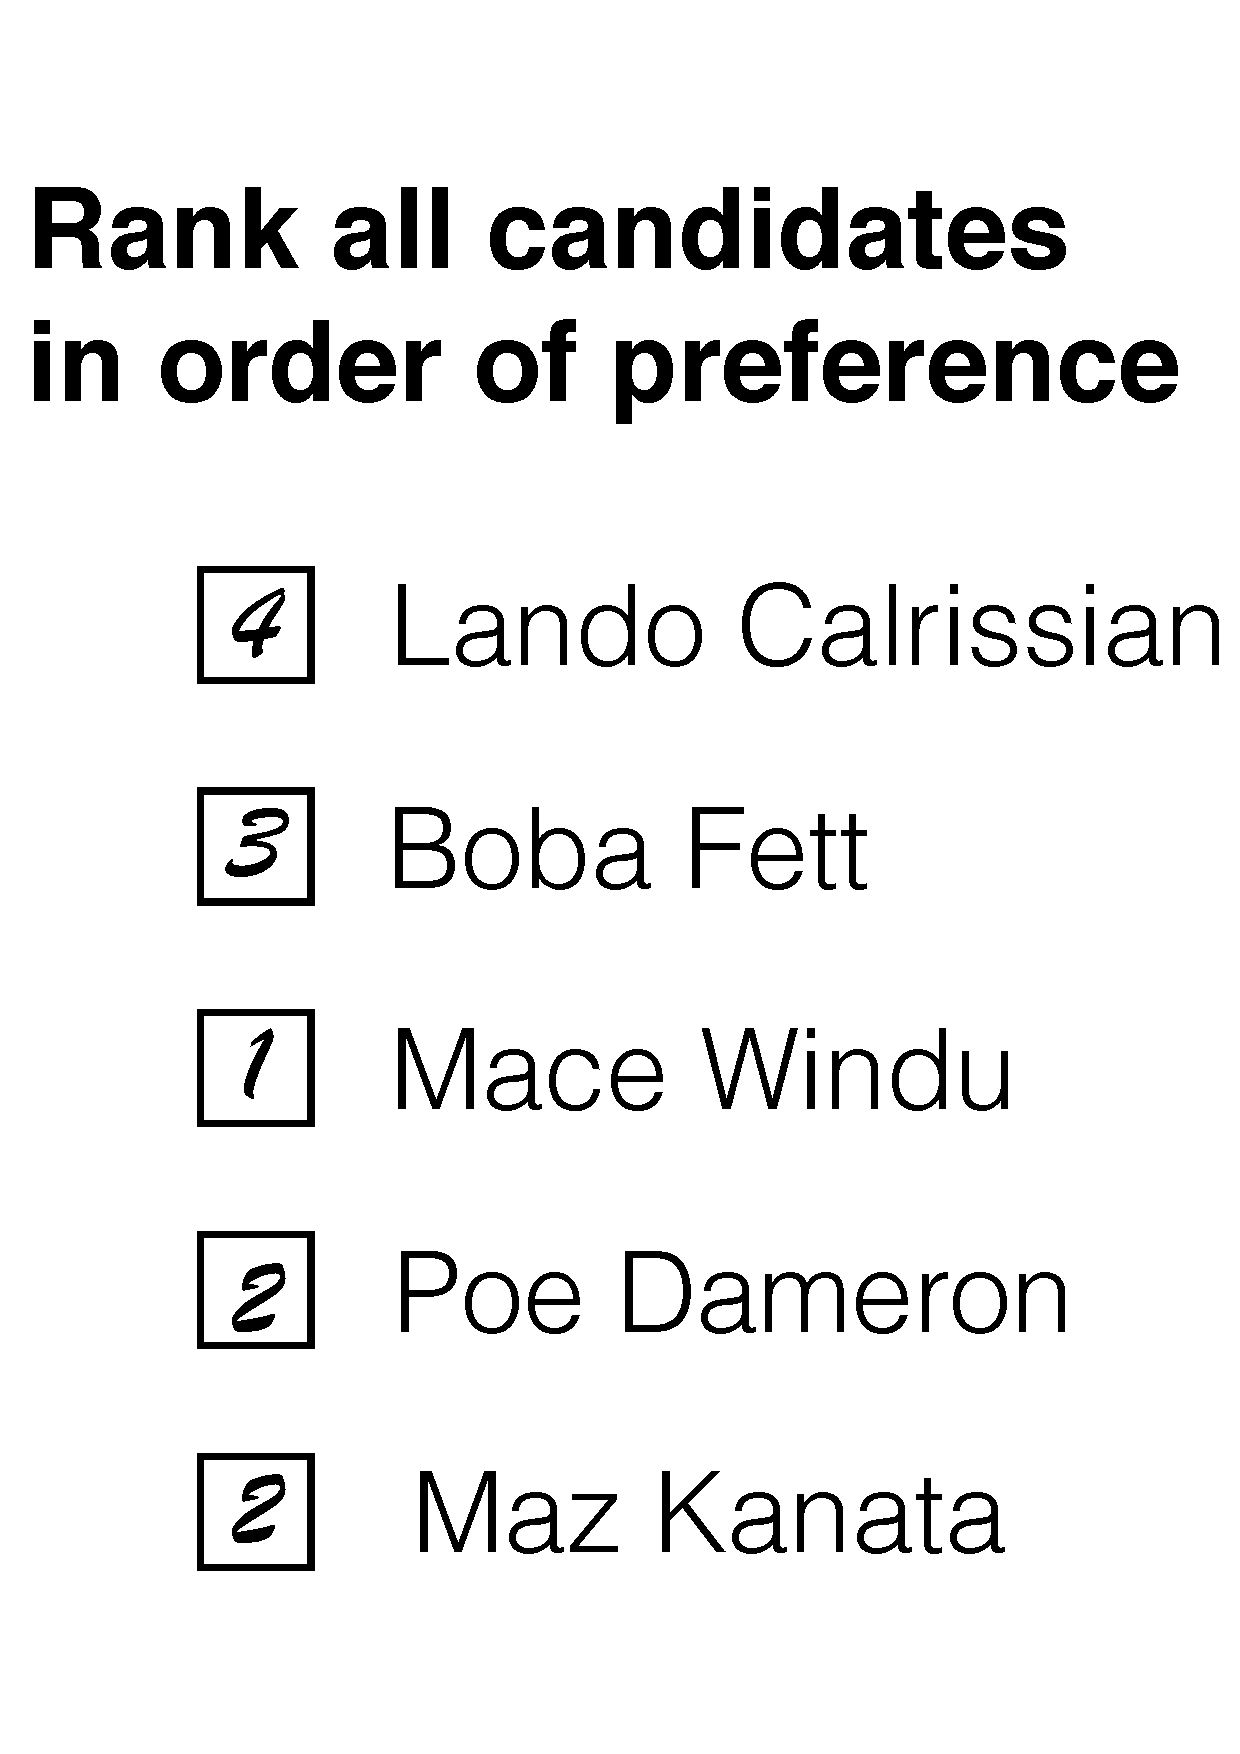
\includegraphics[width=0.37\textwidth]{bal-cropped.pdf}}
    \caption{Ballot Representation}
    \end{center}
\end{figure}
In practice, ballots are
implemented by asking voters to put numerical preferences against
the names of candidates as represented by the image on the right.
The most natural representation of a ballot is therefore a function
$b: C \to Nat$ that assigns a natural number (the preference) for
each candidate, and we recover a strict linear preorder $<_b$ on candidates
by setting $c <_b d$ if $b(c) > b(d)$. 

As preferences are usually
numbered beginning with $1$, we interpret a preference of $0$ as the
voter failing to designate a preference for a candidate
as this allows us to also accommodate incomplete ballots.
This is clearly a design decision, and we could have formalised
ballots as functions $b: C \to 1 + Nat$ (with $1$ being the unit
type) but it would add little to our analysis.
%
%
\begin{verbatim}
  Definition ballot := cand -> nat.
\end{verbatim}

\noindent
The count of an individual election is then parameterised by the list
of ballots cast, and is represented as a dependent inductive type.
More precisely, we have a type \texttt{State} that represents either
an
intermediate stages of constructing the margin function or the
determination of the final election result:
\begin{verbatim}

  Inductive State: Type :=
  | partial: (list ballot * list ballot)  -> (cand -> cand -> Z) -> State
  | winners: (cand -> bool) ->  State.

\end{verbatim}

\noindent
The interpretation of this type is that a state either consists of
two lists of ballots and a margin function, representing

\begin{itemize}
  \item the set of ballots counted so far, and the set of invalid
ballots seen so far
  \item the margin function constructed so far
\end{itemize}
or, to signify that winners have been determined, a boolean function
that determines the set of winners.

The type that formalises correct counting of votes according to the
Schulze method is parameterised by the profile of ballots cast (that
we formalise as a list), and depends on the type \texttt{State}. That
is to say, an inhabitant of the type \texttt{Count n}, for
\texttt{n} of type \texttt{State}, represents a correct execution of
the voting protocol up to reaching state \texttt{n}. This
state generally represents intermediate stages of the construction
of the margin function, with the exception of the final step where
the election winners are being determined. The inductive type takes
the following shape:

\begin{verbatim}
  Inductive Count (bs : list ballot) : State -> Type :=
  | ax us m : us = bs -> (forall c d, m c d = 0) -> 
    Count bs (partial (us, []) m)         (* zero margin      *)
  | cvalid u us m nm inbs : Count bs (partial (u :: us, inbs) m) -> 
    (forall c, (u c > 0)%nat) ->          (* u is valid       *)
    (forall c d : cand, 
      ((u c < u d) -> nm c d = m c d + 1) (* c preferred to d *) /\
      ((u c = u d) -> nm c d = m c d)     (* c, d rank equal  *) /\
      ((u c > u d) -> nm c d = m c d - 1))(* d preferred to c *) ->
    Count bs (partial (us, inbs) nm)
  | cinvalid u us m inbs : Count bs (partial (u :: us, inbs) m) -> 
    (exists c, (u c = 0)%nat)             (* u is invalid     *) ->
    Count bs (partial (us, u :: inbs) m)
  | fin m inbs w (d : (forall c, (wins_type m c) + (loses_type m c))):
    Count bs (partial ([], inbs) m)       (* no ballots left  *) ->
    (forall c, w c = true <-> (exists x, d c = inl x)) ->
    (forall c, w c = false <-> (exists x, d c = inr x)) ->
    Count bs (winners w).
 
\end{verbatim}

\noindent
The intuition here is simple: the first constructor, \texttt{ax},
initiates the construction of the margin function, and we ensure
that all ballots are uncounted, no ballot are invalid (yet), and the
margin function is constantly zero. The second constructor,
\texttt{cvalid}, updates the margin function according to a valid
ballot (all candidates have preferences marked against their name),
and removes the ballot from the list of uncounted ballots. The
constructor \texttt{cinvalid} moves an invalid ballot to the list of
invalid ballots, and the last constructor \texttt{fin} applies only
if the margin function is completely constructed (no more uncounted
ballots). In its arguments, \texttt{w : cand -> bool} is the function
that determines election winners, and \texttt{d} is a function that
delivers, for every candidate, type-level evidence of winning or
losing, consistent with \texttt{w}. Given this, we can conclude the
count and declare \texttt{w} to be the set of winners (or more
precisely, those candidates for which \texttt{w} evaluates to
\texttt{true}).

Together with the equivalence of the propositional notions of
winning or losing a Schulze count with their type-level
counterparts, every inhabitant of the type \texttt{Count b (winners
w)} then represents a correct count of ballots \texttt{b} leading to
the boolean predicate \texttt{w : cand -> bool} that determines the
winners of the election with initial set \texttt{b} of ballots.

The crucial aspect of our formalisation of executions of Schulze
counting is that the transcript of the count is represented by a
type that is \emph{not} a proposition. As a consequence, extraction
delivers a program that produces the (set of) election winner(s),
\emph{together} with the evidence recorded in the type to enable
independent verification.




\subsection{All Schulze Election Have Winners}
\label{sec:all_winners}
The main theorem, the proof of which we describe in this section, is
that all elections according to the Schulze method engender a
boolean-valued function \texttt{w : cand -> bool}
that determines
precisely which candidates are winners of the election, together
with type-level evidence of this.
Note that a Schulze election can have more
than one winner, the simplest (but not the only) example being when
no ballots at all have been cast.
The theorem that we establish (and later extract as a program)
simply states that for every incoming set of ballots, there is a
boolean function that determines the election winners, together with
an inhabitant of the type \texttt{Count} that witnesses the
correctness of the execution of the count. 

\begin{verbatim}
  Theorem schulze_winners: forall (bs : list ballot),
    existsT (w: cand -> bool) (p : Count bs (winners w)), True.
\end{verbatim}


\noindent
The first step in the proof is elementary: We show that for any
given list of ballots we can reach a state of the count where there are
no more uncounted ballots, i.e. the margin function has been
fully constructed.


\begin{verbatim}

  Lemma all_ballots_counted: forall (bs : list ballot), 
     existsT i m, (Count bs (partial ([], i) m)).
        
\end{verbatim}
    
   
   
The second step relies on the iterated margin function already
discussed in Section \ref{sec:prop-type}. As $M_n(c, d)$ (for $n$ being
the number of candidates) is the strength of the strongest path
between $c$ and $d$, we construct a boolean function
$w$ such that $w(c) = \mathtt{true}$ if and only if $M_n(c, d) \geq
M_n(d, c)$ for all $d \in C$. We then construct the type-level
evidence required in the constructor \texttt{fin} 
using  the function (or proposition)
\texttt{iterated\_marg\_wins\_type} described earlier. 


\section{Scrutiny Sheet and Experimental Results}
\label{sec:scrunity_sheet}
	The crucial aspect of our formalisation is that the vote counting
protocol itself is represented as a dependent inductive type
that represents all (correct) partial executions of
the protocol.  A complete execution is can then be understood as a
state of vote counting where election winners have been determined.
Our main theorem, \texttt{schulze\_winners}, then asserts that an 
inhabitant of this type
exists, for all possible sets of incoming ballots. 
Crucially, every such inhabitant contains enough information
to (independently) verify the correctness of the election result,
and can be thought of as a \emph{certificate} for the count.
From a computational perspective, we view tallying not merely as a
function that delivers a result, but instead as a function that
delivers a result, \emph{together} with evidence that allows us to
verify correctness. In other words, we augment verified correctness
of an algorithm with the means to verify each particular
\emph{execution}.


From the perspective of electronic voting, this means that
we no longer need to trust the hardware and software (assuming the 
cast-as-intended and collected-as-cast verifiability)
that was employed to obtain the election result, as the generated
certificate can be verified independently. In the literature on
electronic voting, this is known as (tallied-as-cast) \emph{verifiability} and has
been recognised as one of the cornerstones for building trust in
election outcomes by electronic voting research community \citep{Chaum:2004:SBR}
 \citep{5958051}, \citep{Benaloh:1994:RSE:195058.195407},  \citep{Delaune:2010:VPT}, \citep{Bernhard:2017:PES}.
%and is the only answer to
%key questions such as the possibility of hardware malfunctions, or
%indeed running the very software that has been claimed to count
%votes correctly.
%
%The certificate that is produced by each run of our extracted Schulze vote
%tallying algorithm  consists of two parts. The first part details
%the individual steps of constructing the margin function, based on
%the set of all ballots cast. The second part presents evidence for
%the determination of winners, based on generalised margins. For the
%construction of the margin function, every ballot is processed
%in turn, with the margin between each pair of votes updated
%accordingly.  The heart of our work lies in this second part of the
%certificate. To demonstrate that candidate $c$ is an election
%winner, we have to demonstrate that the generalised margin between
%$c$ and every other candidate $d$ is at least as large than the
%generalised margin  between $d$ and $c$. 
%
%Given that the generalised margin
%between two candidates $c$ and $d$ is determined in terms of
%paths $c, c_1, \dots, c_n, d$ that join $c$
%and $d$, we need to exhibit
%\begin{itemize}
%\item evidence for the existence of a path $p$ from $c$ to $d$
%\item evidence for the fact that \emph{no} path $q$ from $d$ to $c$
%is stronger than $p$
%\end{itemize}
%where the strength of a path $p = (c_0, \dots, c_{n+1})$ is the
%minimum $\min \lbrace m(c_i, c_{i+1}) \mid 0 \leq i \leq n \rbrace$
%of the margins between adjacent nodes. 

%While evidently a path
%itself is evidence for its existence, the \emph{non-existence} of
%paths with certain properties is more difficult to establish. For this,
%we uses a coinductive approach. As existence of a path with a given
%strength between two candidates can be easily phrased as an
%inductive definition, the \emph{complement} of this predicate arises
%as a greatest fixpoint, or equivalently as a coinductively defined
%predicate (see e.g. \citep{Kozen:2016:PC}). This allows us to witness
%the non-existence of paths by exhibiting co-closed sets.
  


Coq's extraction mechanism then allows us to turn our main theorem, 
\linebreak
\texttt{schulze\_winners}, into a
provably correct program. When extracting, all purely propositional
information is erased and given a set of incoming ballots, the ensuing program produces an inhabitant
of the (extracted) type \texttt{Count} that records the construction
of the margin function, together with (type level) evidence of
correctness of the determination of winners. That is, we see the
individual steps of the construction of the margin function (one
step per
ballot) and once all ballots are exhausted, the determination of
winners, together with paths and co-closed sets. The following is
the transcript of a Schulze election where we have added wrappers
to pretty-print the information content. This is the (full) scrutiny
sheet promised in Section \ref{sec:prop-type}.
%
\newpage
\begin{footnotesize}
\begin{verbatim}
V: [A3 B1 C2 D4,..], I: [], M: [AB:0 AC:0 AD:0 BC:0 BD:0 CD:0]
--------------------------------------------------------------
V: [A1 B0 C4 D3,..], I: [], M: [AB:-1 AC:-1 AD:1 BC:1 BD:1 CD:1]
----------------------------------------------------------------
V: [A3 B1 C2 D4,..], I: [A1 B0 C4 D3], M: [AB:-1 AC:-1 AD:1 BC:1 BD:1 CD:1]
---------------------------------------------------------------------------
                     . . .
----------------------------------------------------------------------
V: [A1 B3 C2 D4], I: [A1 B0 C4 D3], M: [AB:2 AC:2 AD:8 BC:5 BD:8 CD:8]
----------------------------------------------------------------------
V: [], I: [A1 B0 C4 D3], M: [AB:3 AC:3 AD:9 BC:4 BD:9 CD:9]
-----------------------------------------------------------
winning: A
  for B: path A --> B of strenght 3, 4-coclosed set: 
    [(B,A),(C,A),(C,B),(D,A),(D,B),(D,C)]
  for C: path A --> C of strenght 3, 4-coclosed set:
    [(B,A),(C,A),(C,B),(D,A),(D,B),(D,C)]
  for D: path A --> D of strenght 9, 10-coclosed set:
    [(D,A),(D,B),(D,C)]
losing: B
  exists A: path A --> B of strength 3, 3-coclosed set:
    [(A,A),(B,A),(B,B),(C,A),(C,B),(C,C),(D,A),(D,B),(D,C),(D,D)]
losing: C
  exists A: path A --> C of strength 3, 3-coclosed set:
    [(A,A),(B,A),(B,B),(C,A),(C,B),(C,C),(D,A),(D,B),(D,C),(D,D)]
losing: D
  exists A: path A --> D of strength 9, 9-coclosed set:
    [(A,A),(A,B),(A,C),(B,A),(B,B),(B,C),(C,A),(C,B),(C,C),(D,A),(D,B),
     (D,C),(D,D)]  
\end{verbatim}
\end{footnotesize}

\noindent
Here, we assume four candidates, \texttt{A}, \texttt{B}, \texttt{C}
and \texttt{D} and a ballot of the form \texttt{A3  B2  C4  D1}
signifies that \texttt{D} is the most preferred candidate (the first
preference), followed by \texttt{B} (second preference), \texttt{A}
and \texttt{C}. In every line, we only display the first uncounted
ballot (condensing the remainder of the ballots to an ellipsis),
followed by votes that we have deemed to be invalid. We display the
partially constructed margin function on the right. Note that the
margin function satisfies  $m(x, y) = -m(y, x)$ and $m(x, x) = 0$ so
that the margins displayed allow us to reconstruct the entire margin
function. In the construction of the margin function, we begin with
the constant zero function, and going from one line to the next, the
new margin function arises by updating according to the first
ballot. This corresponds to the constructor \texttt{cvalid} and
\texttt{cinvalid} being
applied recursively: we see an invalid ballot being set aside in the
step from the second to the third line, all other ballots are valid.
Once the margin function is fully constructed (there are no
more uncounted ballots), we display the evidence provided in the
constructor \texttt{fin}: we present evidence of winning (losing) for
all winning (losing) candidates. 
%
In order to actually verify the computed result, a third party
observer would have to
\begin{enumerate}
\item Check the correctness of the individual steps of computing the
margin function
\item For winners, verify that the claimed paths exist with the
claimed strength, and check that the claimed sets are indeed
coclosed.
\end{enumerate}

\noindent
Contrary to re-running a different implementation on the same
ballots, our scrutiny sheet provides an \emph{orthogonal}
perspective on the data and how it was used to determine the
election result.

We have evaluated our approach by extracting the entire Coq
development into Haskell, with all types defined by Coq extracted as
is, i.e. in particular using Coq's unary representation of natural
numbers. The results are displayed in Figure \ref{fig:test}
using a logarithmic scale. 


%\begin{figure}
%\centering
%\begin{minipage}{.5\textwidth}
%  \centering
%  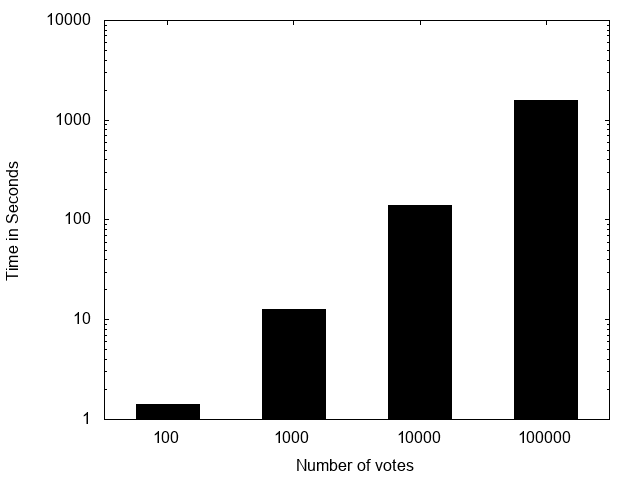
\includegraphics[width=1.0\linewidth]{1.png}
%  \caption{Direct Extraction}
%  \label{fig:straight}
%\end{minipage}
%\begin{minipage}{.5\textwidth}
%  \centering
%  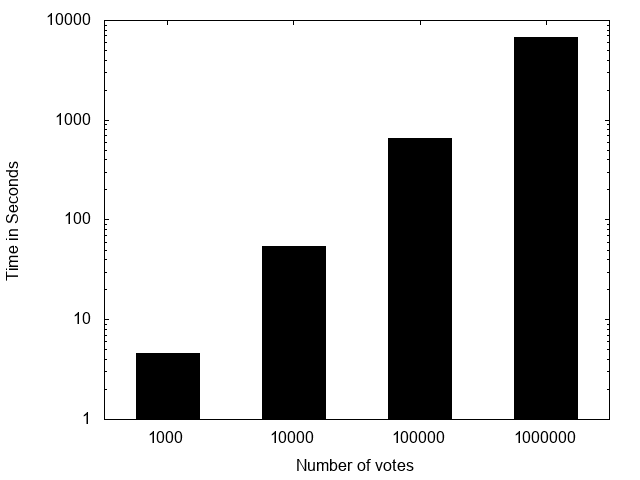
\includegraphics[width=1.0\linewidth]{2.png}
% \caption{Extraction using Haskell Integers}
% \label{fig:native}
%\end{minipage}
%\caption{Experimental Results}
%\label{fig:test}
%\end{figure}


\begin{figure}
\centering     %%% not \center
\subfigure[Direct Extraction]{\label{fig:straightslow}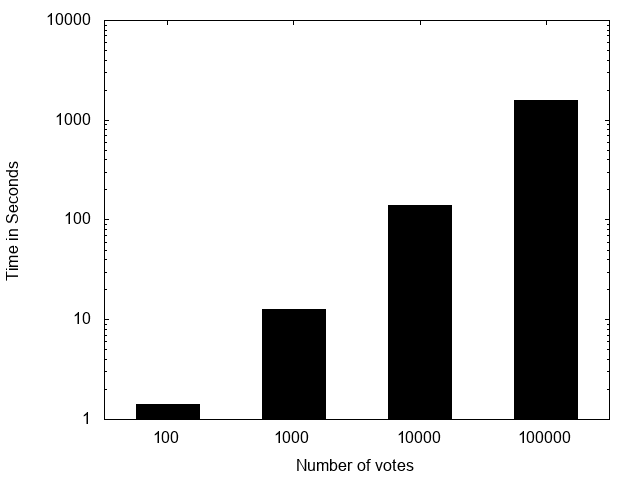
\includegraphics[width=60mm]{1.png}}
\subfigure[Extraction using Haskell Integers]{\label{fig:nativeslow}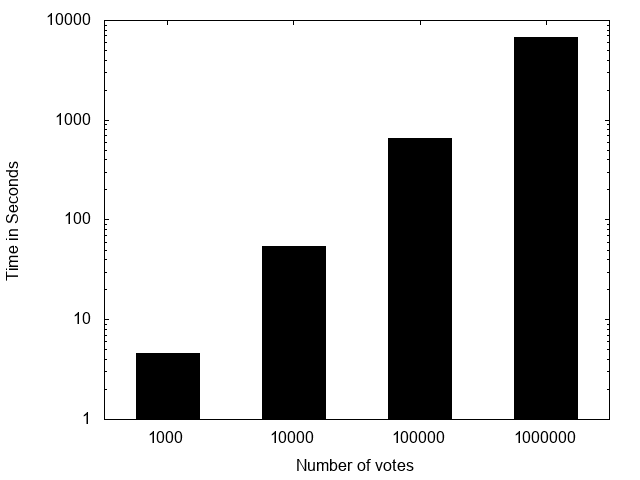
\includegraphics[width=60mm]{2.png}}
\caption{Experimental Results (Slow)}
\label{fig:test}
\end{figure}

%
%\begin{figure}
%\centering
%\begin{subfigure}
%  \centering
%  {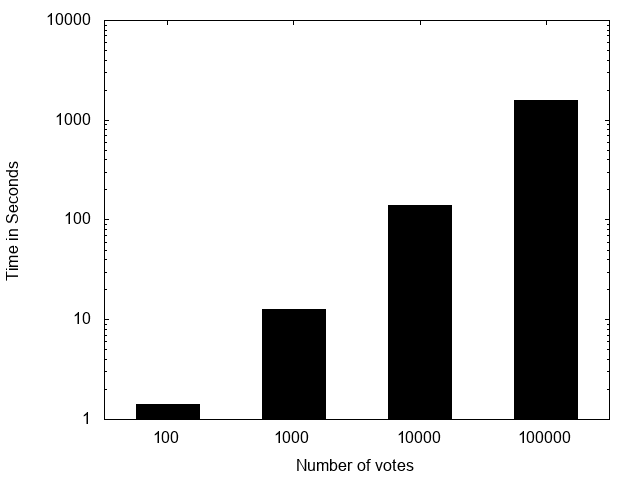
\includegraphics[width=.95\textwidth]{1.png}}
%  \caption{Direct Extraction}
%  \label{fig:straight}
%\end{subfigure}%
%\end{figure}
%\begin{figure}
%\begin{subfigure}
%  \centering
%  {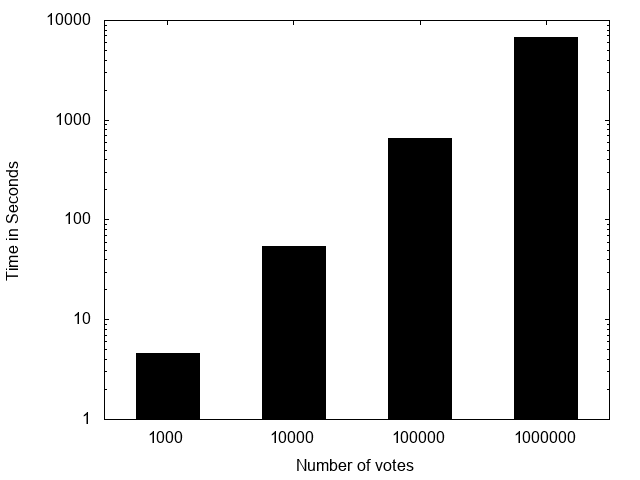
\includegraphics[width=.95\textwidth]{2.png}}
%  \caption{Extraction using Haskell Integers}
%  \label{fig:native}
%\end{subfigure}
%\caption{Experimental Results}
%\label{fig:test}
%\end{figure}
  
 \section{Counting Millions of Ballots}
 \label{sec:count_million}
 The previous extracted Haskell code was very slow  and was not 
 practical for real life election involving millions of ballots. To scale it to real life election,
 we investigated the extracted Haskell code  from Coq code.
The most performance critical aspect of our code was the computation of  margin
function. Recall that the margin function is of type
\texttt{cand -> cand -> Z}
and that it depends on the \emph{entire} set of ballots. Internally, it is
represented by a closure \citep{Landin:1964:MEE} so that margins are
re-computed with every call. The single largest efficiency
improvement in our code was achieved by memoization, i.e.
representing the margin function (in Coq) via list lookup. With
this (and several smaller) optimisation, we can count millions of
votes using verified code. However, this efficiency did not come for 
free, and we had to pay the cost in terms of (almost all) broken proofs. 
We had to redo all the proofs all over again\footnote{Redoing these proofs were trivial,
 but time consuming. I wished if there was a 
tool to automate this process}}.
Below (Figure \ref{fig:fast}), we include our timing graphs,
based on randomly generated ballots while keeping number of candidates
constant i.e. 4 (The reason we kept it to 4 candidate to show the speed up compared to 
 \ref{fig:test}. During the experimentation, we ran an election with 21 candidate, and 
 we were able to count 2 million randomly generated ballots
 before running out of memory.)



\begin{figure}[htb]
\centering     %%% not \center
\subfigure[Computation of Winners]{\label{fig:straightfast}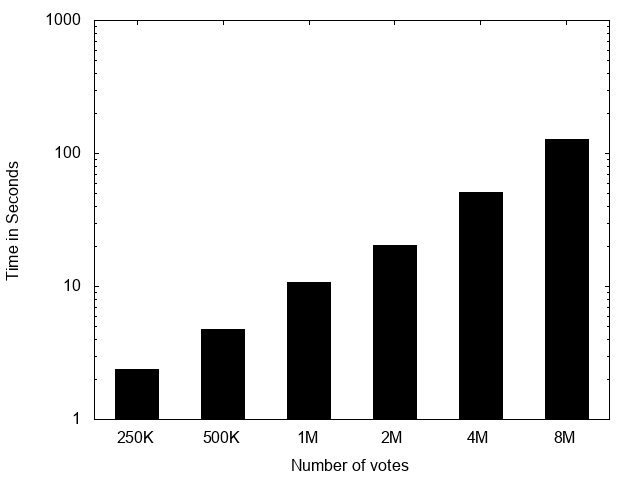
\includegraphics[width=60mm]{without-cert.png}}
\subfigure[Computation of Winners and Certificate]{\label{fig:nativefast}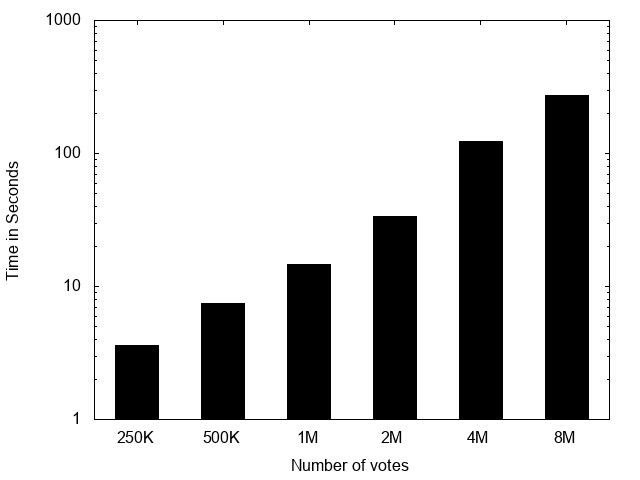
\includegraphics[width=60mm]{with-cert.png}}
\caption{Experimental Results (Fast)}
\label{fig:fast}
\end{figure}


%\begin{figure}
%\centering
%\begin{subfigure}{.5\textwidth}
%  \centering
%  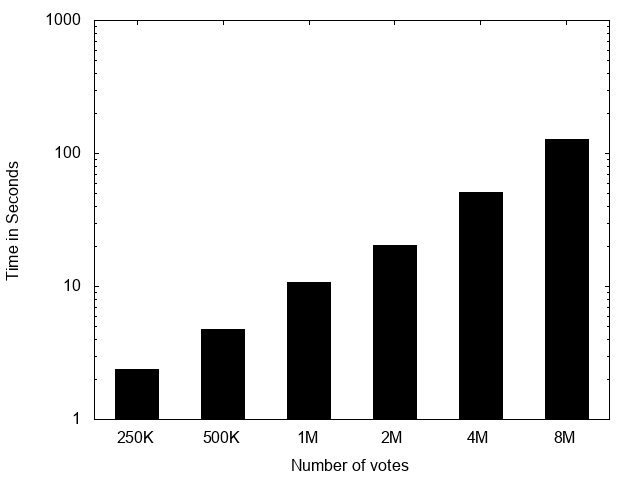
\includegraphics[width=.95\textwidth]{without-cert.png}
%  \caption{Computation of Winners}
%  \label{fig:straight}
%\end{subfigure}%
%\begin{subfigure}{.5\textwidth}
%  \centering
%  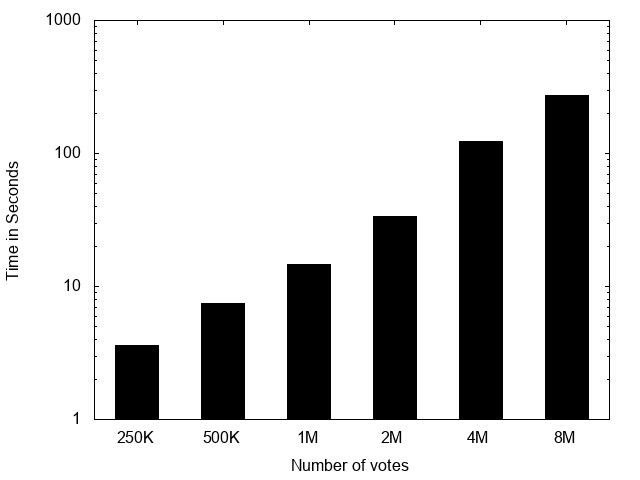
\includegraphics[width=.95\textwidth]{with-cert.png}
%  \caption{Computation of Winners and Certificate}
%  \label{fig:native}
%\end{subfigure}
%\caption{Experimental Results}
%\end{figure}

\noindent
On the left, we report timings (in seconds) for the computation of
winners, whereas on the right, we include the time to additionally
compute a universally verifiable certificate that attests  to the
correctness of the count. This is consistent with complexity of Schulze 
counting i.e. linear in no of ballots and cubic in candidates. 
The experiments were carried out on system 
equipped with intel core i7 processor and 16 GB of ram. We notice that the
computation of the certiciate adds comparatively little in
computational cost. 

Our implementation requires that we store \emph{all}
ballots in main memory as we need to parse the entire list of
ballots before making it available to our verified implementation so
that the total number of ballots we can count is limited by main
memory in practise. We can count real-world size elections (8
million ballot papers) on a standard, commodity desktop computer with
16 GB of main memory. 

  
\section{Discussion} \label{sec:discussion}

In this chapter,  we emphasize on correctness, 
and we take the approach that computation of winners in
electronic voting (and in situations where correctness is key in
general) should not only produce an end result, but an end result,
\emph{together} with a verifiable justification of the correctness
of the computed result. We have exemplified this
approach by providing a provably correct, and evidence-producing
implementation of vote counting according to the Schulze method. 

While the Schulze method is not difficult to implement, and indeed
there are many freely available implementations on the Internet, 
comparing the
results between different implementations can give some level of
assurance for correctness only in case the results agree.  If there
is a discrepancy, a certificate for the correctness of the count
allows to adjudicate between different implementations, as the
certificate can be checked with relatively little computational
effort. 

From the perspective of computational complexity, checking a
transcript for correctness is of the same complexity as computing
the set of winners, as our certificates are cubic in size, so that
certificate checking is not less complex than the actual
computation. 
However, publishing an independently verifiable certificate that
attests the individual steps of the computation helps to increase
\emph{trust} in the computed election outcome. Typically, the use of technology in
elections increases the amount of trust that we need to place both
in technological artefacts, and in people. It raises questions that
range from fundamental aspects, such as proper testing and/or
verification of the software, to very practical questions, e.g.
whether the correct version of the software has been run.  On the
contrast, publishing a certificate of the count dramatically reduces
the amount of trust that we need to place into both people and
technology: the ability to publish a verifiable justification of the
correctness of the count allows a large number of individuals to
scrutinise the count. While only moderate programming skills are
required to check the validity of a certificate (the transcript of
the count), even individuals without any programming background can
at least spot-check the transcript: for the construction of the
margin function, everything that is needed is to show that the
respective margins change according to the counted ballot. For the
correctness of determination of winners, it is easy to verify
existence of paths of a given strength, and also whether certain
sets are co-closed -- even by hand! This dramatically increases the
class of people that can scrutinise the correctness of the count,
and so helps to establish a trust basis that is much wider as no
trust in election officials and software artefacts is required.


Technically, we do not \emph{implement} an algorithm that counts
votes according to the Schulze method. Instead, we give a
specification of the Schulze winning conditions 
(\texttt{wins\_prop} in  Section \ref{sec:spec}) in terms of an
already computed margin function that
(we hope) can immediately be seen to be correct, and then show that those
winning conditions are equivalent to the existence of inhabitants of
types that carry verifiable evidence (\texttt{wins\_type}).  We then
join the (type level) winning conditions with an inductive type that
details the construction of the margin function in an inductive
type. Via propositions-as-types, a provably correct vote counting
function is then equivalent the proposition that there exists an
inhabitant of \texttt{Count} for every set of ballots.  Coq's
extraction mechanism then allows us to extract a Haskell program
that produces election winners, together with verifiable
certificates. 

\section{Summary}

Our formalization achieves \textit{Correctness}, \textit{Practicality}, and 
(tallied-as-cast) \textit{Verifiability}. The major problem in this formalization is \textit{Privacy}.  
Our ballots are in plaintext and could easily be identified
if the number of candidates participating in election in 
are large (Italian attack) \citep{Otten}.
\noindent
In nutshell, the achieved and missed of this formalization:

\begin{itemize}
\item Achieved 
\begin{itemize}
\item Correctness: The implementation is formalized in Coq with emphasis on generating 
         evidence to convince everyone about the outcome of election.
\item Practicality: The extracted code can count millions of ballots. Therefore, we can use it 
          in any real life election.
\item Verifiability: The outcome of any election can be verified by any third party using 
		  the generated certificates. Certificates generated for plaintext ballot 
		  during the election 
          are very simple.  It requires basic math literacy to audit the certificate which would 
          lead to increase in number of scrutineers. 

\end{itemize}
\item Missed
\begin{itemize}
\item Privacy: There is no privacy  because the ballots involved 
         are simply plaintext, and potentially, it could lead coercion and vote-selling (coercion).
\end{itemize}
\end{itemize}

We remark that extracting Coq developments into a
programming language itself is a non-verified process which could
still introduce errors in our code. The most promising way to
alleviate this is to independently implement (and verify) a
certificate verifier, possibly in a language such as CakeML
\citep{Kumar:2014:CVI} that is guaranteed to
be correct to the machine level. 

 In the next chapter, we will try to solve privacy and coercion problem, using encryption, and to keep 
 it verifiable, we will use zero-knowledge-proof. However, solution for privacy comes at cost, e.g. 
 a loss in the pool of scrutineers because auditing a certificate generated by counting encrypted ballot 
 would requires intricate knowledge of cryptography.
 

